\documentclass[a4paper]{book}
\usepackage{makeidx}
\usepackage{graphicx}
\usepackage{multicol}
\usepackage{float}
\usepackage{listings}
\usepackage{color}
\usepackage{ifthen}
\usepackage[table]{xcolor}
\usepackage{textcomp}
\usepackage{alltt}
\usepackage{ifpdf}
\ifpdf
\usepackage[pdftex,
            pagebackref=true,
            colorlinks=true,
            linkcolor=blue,
            unicode
           ]{hyperref}
\else
\usepackage[ps2pdf,
            pagebackref=true,
            colorlinks=true,
            linkcolor=blue,
            unicode
           ]{hyperref}
\usepackage{pspicture}
\fi
\usepackage[utf8]{inputenc}
\usepackage{mathptmx}
\usepackage[scaled=.90]{helvet}
\usepackage{courier}
\usepackage{doxygen}
\lstset{language=C++,inputencoding=utf8,basicstyle=\footnotesize,breaklines=true,breakatwhitespace=true,tabsize=8,numbers=left }
\makeindex
\setcounter{tocdepth}{3}
\renewcommand{\footrulewidth}{0.4pt}
\begin{document}
\hypersetup{pageanchor=false}
\begin{titlepage}
\vspace*{7cm}
\begin{center}
{\Large Reference Manual}\\
\vspace*{1cm}
{\large Generated by Doxygen 1.7.3}\\
\vspace*{0.5cm}
{\small Mon Jan 2 2012 17:16:17}\\
\end{center}
\end{titlepage}
\clearemptydoublepage
\pagenumbering{roman}
\tableofcontents
\clearemptydoublepage
\pagenumbering{arabic}
\hypersetup{pageanchor=true}
\chapter{Namespace Index}
\section{Namespace List}
Here is a list of all documented namespaces with brief descriptions:\begin{DoxyCompactList}
\item\contentsline{section}{\hyperlink{namespaceUi}{Ui} (Namespace ui is generate by qt for make the code lighter )}{\pageref{namespaceUi}}{}
\end{DoxyCompactList}

\chapter{Class Index}
\section{Class Hierarchy}
This inheritance list is sorted roughly, but not completely, alphabetically:\begin{DoxyCompactList}
\item \contentsline{section}{DialogAjout}{\pageref{classDialogAjout}}{}
\item \contentsline{section}{DialogManuel}{\pageref{classDialogManuel}}{}
\item \contentsline{section}{DialogSuppr}{\pageref{classDialogSuppr}}{}
\item \contentsline{section}{Document}{\pageref{classDocument}}{}
\begin{DoxyCompactList}
\item \contentsline{section}{Livre}{\pageref{classLivre}}{}
\begin{DoxyCompactList}
\item \contentsline{section}{Article}{\pageref{classArticle}}{}
\item \contentsline{section}{BD}{\pageref{classBD}}{}
\begin{DoxyCompactList}
\item \contentsline{section}{Comic}{\pageref{classComic}}{}
\item \contentsline{section}{Manga}{\pageref{classManga}}{}
\end{DoxyCompactList}
\item \contentsline{section}{Roman}{\pageref{classRoman}}{}
\end{DoxyCompactList}
\end{DoxyCompactList}
\item \contentsline{section}{Gestionnaire}{\pageref{classGestionnaire}}{}
\end{DoxyCompactList}

\chapter{Class Index}
\section{Class List}
Here are the classes, structs, unions and interfaces with brief descriptions:\begin{DoxyCompactList}
\item\contentsline{section}{\hyperlink{classArticle}{Article} (Class \hyperlink{classArticle}{Article}, inheriting of class \hyperlink{classLivre}{Livre} )}{\pageref{classArticle}}{}
\item\contentsline{section}{\hyperlink{classBD}{BD} (Class \hyperlink{classBD}{BD}, inheriting of class \hyperlink{classLivre}{Livre} )}{\pageref{classBD}}{}
\item\contentsline{section}{\hyperlink{classComic}{Comic} (Class \hyperlink{classComic}{Comic}, inheriting of class \hyperlink{classBD}{BD} )}{\pageref{classComic}}{}
\item\contentsline{section}{\hyperlink{classDialogAjout}{DialogAjout} (Class \hyperlink{classDialogAjout}{DialogAjout}, inheriting of class QDialog )}{\pageref{classDialogAjout}}{}
\item\contentsline{section}{\hyperlink{classDialogManuel}{DialogManuel} (Class \hyperlink{classDialogManuel}{DialogManuel}, inheriting of class QDialog )}{\pageref{classDialogManuel}}{}
\item\contentsline{section}{\hyperlink{classDialogSuppr}{DialogSuppr} (Class \hyperlink{classDialogSuppr}{DialogSuppr}, inheriting of class QDialog )}{\pageref{classDialogSuppr}}{}
\item\contentsline{section}{\hyperlink{classDocument}{Document} (Class \hyperlink{classDocument}{Document}, mother class of all document's type classes )}{\pageref{classDocument}}{}
\item\contentsline{section}{\hyperlink{classGestionnaire}{Gestionnaire} (Class \hyperlink{classGestionnaire}{Gestionnaire}, inheriting of class QMainWindow, it is the main window of the programme )}{\pageref{classGestionnaire}}{}
\item\contentsline{section}{\hyperlink{classLivre}{Livre} (Class \hyperlink{classLivre}{Livre}, inheriting of class \hyperlink{classDocument}{Document} )}{\pageref{classLivre}}{}
\item\contentsline{section}{\hyperlink{classManga}{Manga} (Class \hyperlink{classManga}{Manga}, inheriting of class \hyperlink{classBD}{BD} )}{\pageref{classManga}}{}
\item\contentsline{section}{\hyperlink{classRoman}{Roman} (Class \hyperlink{classRoman}{Roman}, inheriting of class \hyperlink{classLivre}{Livre} )}{\pageref{classRoman}}{}
\end{DoxyCompactList}

\chapter{Namespace Documentation}
\hypertarget{namespaceUi}{
\section{Ui Namespace Reference}
\label{namespaceUi}\index{Ui@{Ui}}
}


namespace ui is generate by qt for make the code lighter  




\subsection{Detailed Description}
namespace ui is generate by qt for make the code lighter 
\chapter{Class Documentation}
\hypertarget{classArticle}{
\section{Article Class Reference}
\label{classArticle}\index{Article@{Article}}
}


class \hyperlink{classArticle}{Article}, inheriting of class \hyperlink{classLivre}{Livre}  




{\ttfamily \#include $<$article.hh$>$}

Inheritance diagram for Article:\begin{figure}[H]
\begin{center}
\leavevmode
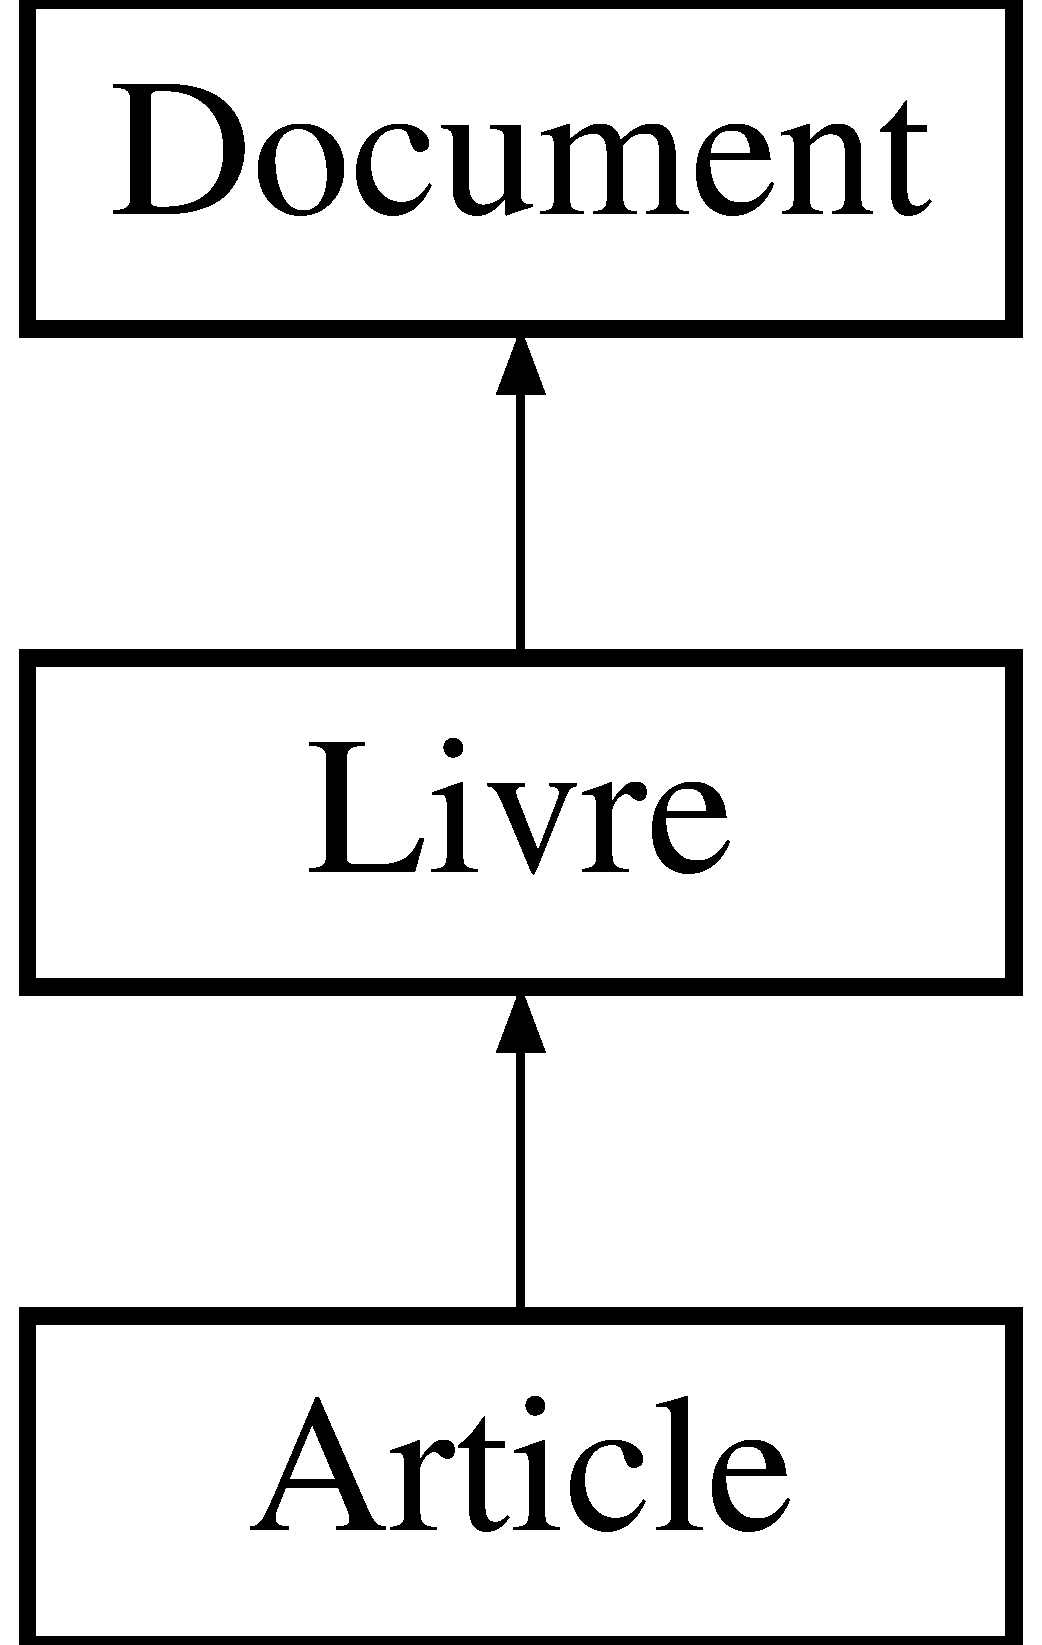
\includegraphics[height=3.000000cm]{classArticle}
\end{center}
\end{figure}
\subsection*{Public Member Functions}
\begin{DoxyCompactItemize}
\item 
\hypertarget{classArticle_a58990f0362ae7e950e1a1d4f4b9f9453}{
void \hyperlink{classArticle_a58990f0362ae7e950e1a1d4f4b9f9453}{setTheme} (const std::string \&)}
\label{classArticle_a58990f0362ae7e950e1a1d4f4b9f9453}

\begin{DoxyCompactList}\small\item\em function setTheme who set the theme of an article \item\end{DoxyCompactList}\item 
\hypertarget{classArticle_a2d927194ffdd4c66021adb5fabe0da40}{
std::string \hyperlink{classArticle_a2d927194ffdd4c66021adb5fabe0da40}{getTheme} ()}
\label{classArticle_a2d927194ffdd4c66021adb5fabe0da40}

\begin{DoxyCompactList}\small\item\em function getTheme who return the theme of an article \item\end{DoxyCompactList}\item 
\hypertarget{classArticle_a00ee1ebbaf5e559732933dd29f0a9360}{
void \hyperlink{classArticle_a00ee1ebbaf5e559732933dd29f0a9360}{setDateParution} (const std::string \&)}
\label{classArticle_a00ee1ebbaf5e559732933dd29f0a9360}

\begin{DoxyCompactList}\small\item\em function setDateParution who set the date of parution of an article \item\end{DoxyCompactList}\item 
\hypertarget{classArticle_a0c97939e7c98396fbe68bd32509470bf}{
std::string \hyperlink{classArticle_a0c97939e7c98396fbe68bd32509470bf}{getDateParution} ()}
\label{classArticle_a0c97939e7c98396fbe68bd32509470bf}

\begin{DoxyCompactList}\small\item\em function getDateParution who return the date of parution of an article \item\end{DoxyCompactList}\end{DoxyCompactItemize}
\subsection*{Protected Attributes}
\begin{DoxyCompactItemize}
\item 
\hypertarget{classArticle_abfa5c99c0ced717090470e7767c9966f}{
std::string {\bfseries \_\-theme}}
\label{classArticle_abfa5c99c0ced717090470e7767c9966f}

\item 
\hypertarget{classArticle_a9769e51b548f0a8216113ab00db9f71c}{
std::string {\bfseries \_\-dateParution}}
\label{classArticle_a9769e51b548f0a8216113ab00db9f71c}

\end{DoxyCompactItemize}


\subsection{Detailed Description}
class \hyperlink{classArticle}{Article}, inheriting of class \hyperlink{classLivre}{Livre} 

The documentation for this class was generated from the following files:\begin{DoxyCompactItemize}
\item 
article.hh\item 
article.cpp\end{DoxyCompactItemize}

\hypertarget{classBD}{
\section{BD Class Reference}
\label{classBD}\index{BD@{BD}}
}


class \hyperlink{classBD}{BD}, inheriting of class \hyperlink{classLivre}{Livre}  




{\ttfamily \#include $<$bd.hh$>$}

Inheritance diagram for BD:\begin{figure}[H]
\begin{center}
\leavevmode
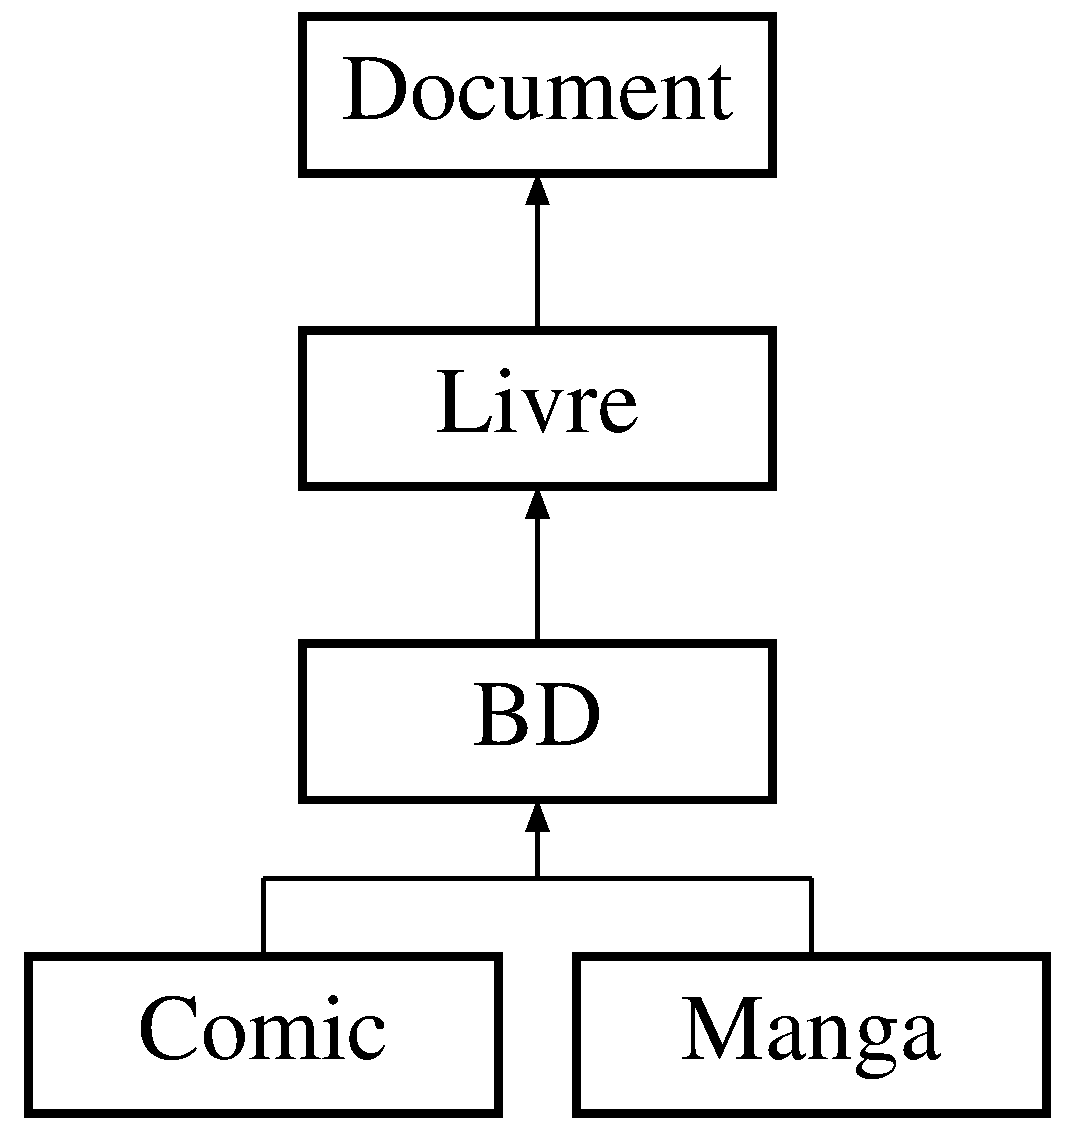
\includegraphics[height=4.000000cm]{classBD}
\end{center}
\end{figure}
\subsection*{Public Member Functions}
\begin{DoxyCompactItemize}
\item 
\hypertarget{classBD_ab2f657f8370b98b5d48789e89ff886f2}{
void \hyperlink{classBD_ab2f657f8370b98b5d48789e89ff886f2}{setEditor} (const std::string \&)}
\label{classBD_ab2f657f8370b98b5d48789e89ff886f2}

\begin{DoxyCompactList}\small\item\em function setEditor who set the editor of a \hyperlink{classBD}{BD} \item\end{DoxyCompactList}\item 
\hypertarget{classBD_a5d3c1d418d7907616b8febd605284741}{
std::string \hyperlink{classBD_a5d3c1d418d7907616b8febd605284741}{getEditor} ()}
\label{classBD_a5d3c1d418d7907616b8febd605284741}

\begin{DoxyCompactList}\small\item\em function getEditor who return the editor of a \hyperlink{classBD}{BD} \item\end{DoxyCompactList}\end{DoxyCompactItemize}
\subsection*{Protected Attributes}
\begin{DoxyCompactItemize}
\item 
\hypertarget{classBD_ac9bd35f0626ee0d32b97ec7467dce17c}{
std::string {\bfseries \_\-editor}}
\label{classBD_ac9bd35f0626ee0d32b97ec7467dce17c}

\end{DoxyCompactItemize}


\subsection{Detailed Description}
class \hyperlink{classBD}{BD}, inheriting of class \hyperlink{classLivre}{Livre} 

The documentation for this class was generated from the following files:\begin{DoxyCompactItemize}
\item 
bd.hh\item 
bd.cpp\end{DoxyCompactItemize}

\hypertarget{classComic}{
\section{Comic Class Reference}
\label{classComic}\index{Comic@{Comic}}
}


class \hyperlink{classComic}{Comic}, inheriting of class \hyperlink{classBD}{BD}  




{\ttfamily \#include $<$comic.hh$>$}

Inheritance diagram for Comic:\begin{figure}[H]
\begin{center}
\leavevmode
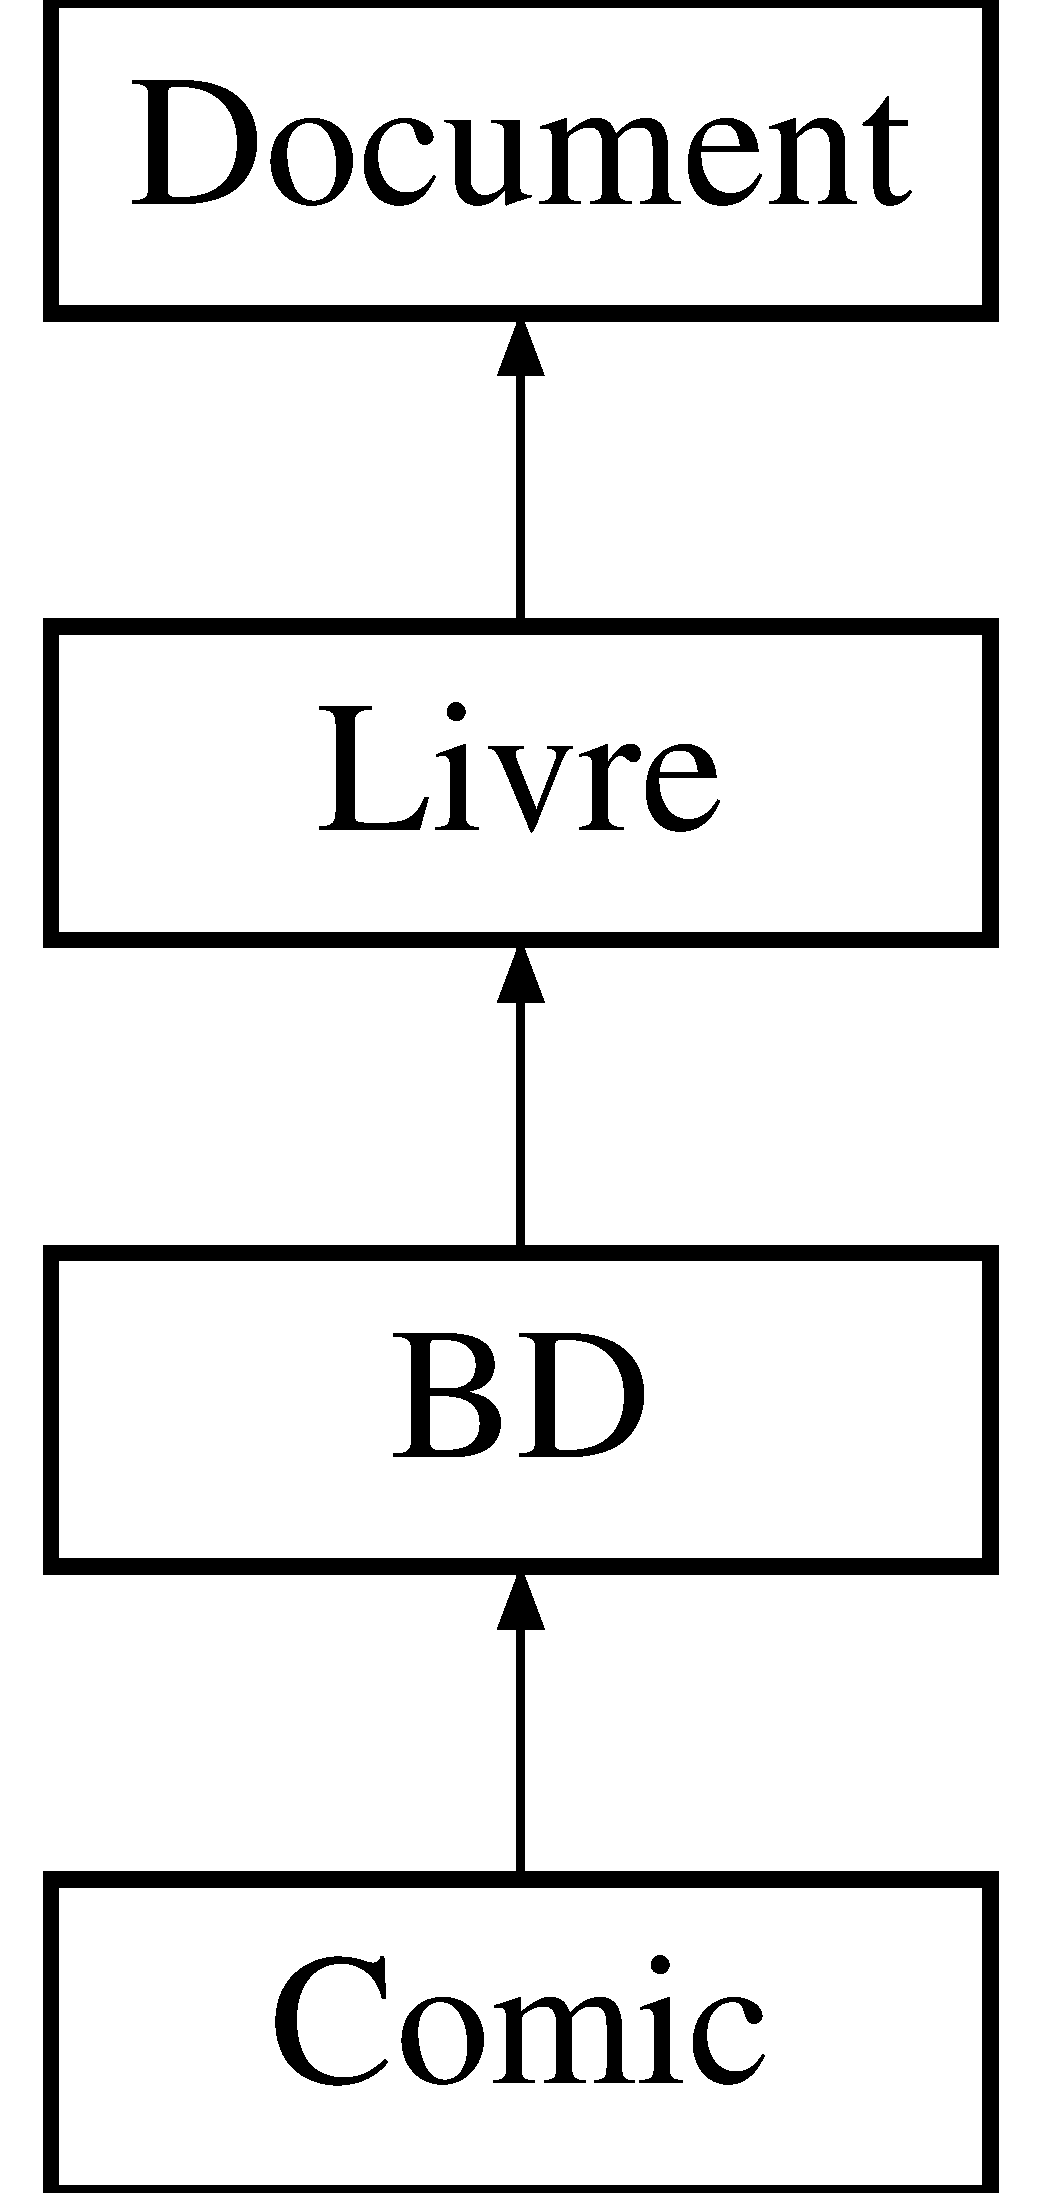
\includegraphics[height=4.000000cm]{classComic}
\end{center}
\end{figure}


\subsection{Detailed Description}
class \hyperlink{classComic}{Comic}, inheriting of class \hyperlink{classBD}{BD} 

The documentation for this class was generated from the following files:\begin{DoxyCompactItemize}
\item 
comic.hh\item 
comic.cpp\end{DoxyCompactItemize}

\hypertarget{classDialogAjout}{
\section{DialogAjout Class Reference}
\label{classDialogAjout}\index{DialogAjout@{DialogAjout}}
}


class \hyperlink{classDialogAjout}{DialogAjout}, inheriting of class QDialog  




{\ttfamily \#include $<$dialogajout.h$>$}

\subsection*{Public Member Functions}
\begin{DoxyCompactItemize}
\item 
\hypertarget{classDialogAjout_aaeabc0c9e541d0f18de919d2fea1a1a3}{
{\bfseries DialogAjout} (QWidget $\ast$parent=0)}
\label{classDialogAjout_aaeabc0c9e541d0f18de919d2fea1a1a3}

\item 
void \hyperlink{classDialogAjout_a72cebaf0d6182830a4a31c24b32911a8}{sauvegarde} ()
\begin{DoxyCompactList}\small\item\em function sauvegarde in \hyperlink{classDialogAjout}{DialogAjout} \item\end{DoxyCompactList}\item 
\hypertarget{classDialogAjout_acf81308622f54b686f629f87281e1051}{
std::string \hyperlink{classDialogAjout_acf81308622f54b686f629f87281e1051}{getTitle} ()}
\label{classDialogAjout_acf81308622f54b686f629f87281e1051}

\begin{DoxyCompactList}\small\item\em function getTitle whoe return the title of the new \hyperlink{classDocument}{Document}. \item\end{DoxyCompactList}\item 
\hypertarget{classDialogAjout_ae98149a8e53298df2c78f777fae0febd}{
std::string \hyperlink{classDialogAjout_ae98149a8e53298df2c78f777fae0febd}{getCat} ()}
\label{classDialogAjout_ae98149a8e53298df2c78f777fae0febd}

\begin{DoxyCompactList}\small\item\em function getCat who return the categorie of the new \hyperlink{classDocument}{Document}. \item\end{DoxyCompactList}\end{DoxyCompactItemize}


\subsection{Detailed Description}
class \hyperlink{classDialogAjout}{DialogAjout}, inheriting of class QDialog 

\subsection{Member Function Documentation}
\hypertarget{classDialogAjout_a72cebaf0d6182830a4a31c24b32911a8}{
\index{DialogAjout@{DialogAjout}!sauvegarde@{sauvegarde}}
\index{sauvegarde@{sauvegarde}!DialogAjout@{DialogAjout}}
\subsubsection[{sauvegarde}]{\setlength{\rightskip}{0pt plus 5cm}void DialogAjout::sauvegarde (
\begin{DoxyParamCaption}
{}
\end{DoxyParamCaption}
)}}
\label{classDialogAjout_a72cebaf0d6182830a4a31c24b32911a8}


function sauvegarde in \hyperlink{classDialogAjout}{DialogAjout} 



open a file in writing

insert lines in the file opened

close the file

open a file in writing

insert lines in the file opened

close the file

open a file in writing

insert lines in the file opened

close the file

open a file in writing

insert lines in the file opened

close the file 



The documentation for this class was generated from the following files:\begin{DoxyCompactItemize}
\item 
dialogajout.h\item 
dialogajout.cpp\end{DoxyCompactItemize}

\hypertarget{classDialogManuel}{
\section{DialogManuel Class Reference}
\label{classDialogManuel}\index{DialogManuel@{DialogManuel}}
}


class \hyperlink{classDialogManuel}{DialogManuel}, inheriting of class QDialog  




{\ttfamily \#include $<$dialogmanuel.hh$>$}

\subsection*{Public Member Functions}
\begin{DoxyCompactItemize}
\item 
\hypertarget{classDialogManuel_ab4b4b79e73df6c879d7384a874ed6226}{
{\bfseries DialogManuel} (QWidget $\ast$parent=0)}
\label{classDialogManuel_ab4b4b79e73df6c879d7384a874ed6226}

\end{DoxyCompactItemize}
\subsection*{Protected Member Functions}
\begin{DoxyCompactItemize}
\item 
\hypertarget{classDialogManuel_ac2310eeebe9d185268b5799cecb3a712}{
void {\bfseries changeEvent} (QEvent $\ast$e)}
\label{classDialogManuel_ac2310eeebe9d185268b5799cecb3a712}

\end{DoxyCompactItemize}


\subsection{Detailed Description}
class \hyperlink{classDialogManuel}{DialogManuel}, inheriting of class QDialog 

The documentation for this class was generated from the following files:\begin{DoxyCompactItemize}
\item 
dialogmanuel.hh\item 
dialogmanuel.cpp\end{DoxyCompactItemize}

\hypertarget{classDialogSuppr}{
\section{DialogSuppr Class Reference}
\label{classDialogSuppr}\index{DialogSuppr@{DialogSuppr}}
}


class \hyperlink{classDialogSuppr}{DialogSuppr}, inheriting of class QDialog  




{\ttfamily \#include $<$dialogsuppr.hh$>$}

\subsection*{Public Member Functions}
\begin{DoxyCompactItemize}
\item 
\hypertarget{classDialogSuppr_affbe6fa75215bb1bf4f35b89de101e2d}{
{\bfseries DialogSuppr} (QWidget $\ast$parent=0)}
\label{classDialogSuppr_affbe6fa75215bb1bf4f35b89de101e2d}

\item 
\hypertarget{classDialogSuppr_a56dc789c9e5f42dd71e9ff37ad497c3e}{
std::string \hyperlink{classDialogSuppr_a56dc789c9e5f42dd71e9ff37ad497c3e}{getTitle} ()}
\label{classDialogSuppr_a56dc789c9e5f42dd71e9ff37ad497c3e}

\begin{DoxyCompactList}\small\item\em function getTitle who return the title of the file to delete \item\end{DoxyCompactList}\item 
\hypertarget{classDialogSuppr_a46ed4e9bf7cefe40670c4df3b4cb637a}{
std::string \hyperlink{classDialogSuppr_a46ed4e9bf7cefe40670c4df3b4cb637a}{getCat} ()}
\label{classDialogSuppr_a46ed4e9bf7cefe40670c4df3b4cb637a}

\begin{DoxyCompactList}\small\item\em function getCat who return the type of the file to delete \item\end{DoxyCompactList}\end{DoxyCompactItemize}
\subsection*{Protected Member Functions}
\begin{DoxyCompactItemize}
\item 
\hypertarget{classDialogSuppr_a098e0e2b472f81bb740ccda02cf8cecd}{
void {\bfseries changeEvent} (QEvent $\ast$e)}
\label{classDialogSuppr_a098e0e2b472f81bb740ccda02cf8cecd}

\end{DoxyCompactItemize}


\subsection{Detailed Description}
class \hyperlink{classDialogSuppr}{DialogSuppr}, inheriting of class QDialog 

The documentation for this class was generated from the following files:\begin{DoxyCompactItemize}
\item 
dialogsuppr.hh\item 
dialogsuppr.cpp\end{DoxyCompactItemize}

\hypertarget{classDocument}{
\section{Document Class Reference}
\label{classDocument}\index{Document@{Document}}
}


class \hyperlink{classDocument}{Document}, mother class of all document's type classes.  




{\ttfamily \#include $<$document.hh$>$}

Inheritance diagram for Document:\begin{figure}[H]
\begin{center}
\leavevmode
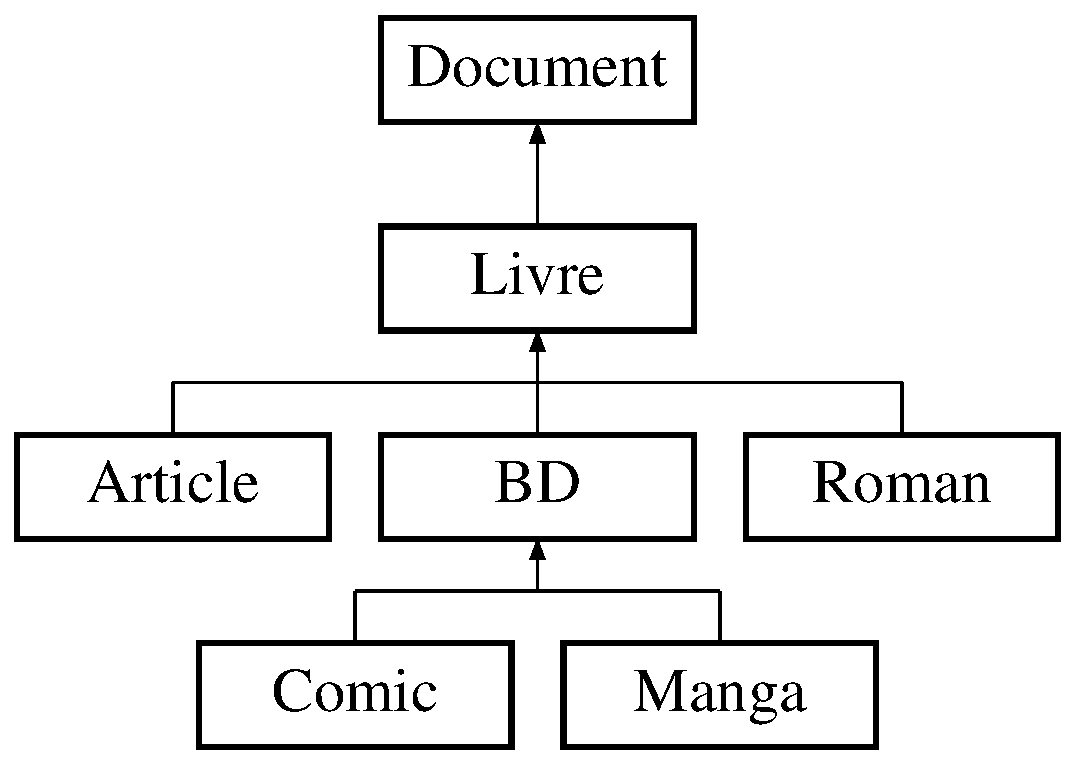
\includegraphics[height=4.000000cm]{classDocument}
\end{center}
\end{figure}
\subsection*{Public Member Functions}
\begin{DoxyCompactItemize}
\item 
\hypertarget{classDocument_a2be00cdaa69a39d54b5238211d0583de}{
void \hyperlink{classDocument_a2be00cdaa69a39d54b5238211d0583de}{setTitle} (const std::string \&)}
\label{classDocument_a2be00cdaa69a39d54b5238211d0583de}

\begin{DoxyCompactList}\small\item\em function setTitle who set the title of a \hyperlink{classDocument}{Document} \item\end{DoxyCompactList}\item 
\hypertarget{classDocument_a6f9dfdb78146953a8cead4c186dff027}{
std::string \hyperlink{classDocument_a6f9dfdb78146953a8cead4c186dff027}{getTitle} ()}
\label{classDocument_a6f9dfdb78146953a8cead4c186dff027}

\begin{DoxyCompactList}\small\item\em function getTitle who return the title of a \hyperlink{classDocument}{Document} \item\end{DoxyCompactList}\end{DoxyCompactItemize}
\subsection*{Protected Attributes}
\begin{DoxyCompactItemize}
\item 
\hypertarget{classDocument_ac21a0c8503c8f62484fcbe319aa3c754}{
std::string {\bfseries \_\-title}}
\label{classDocument_ac21a0c8503c8f62484fcbe319aa3c754}

\end{DoxyCompactItemize}


\subsection{Detailed Description}
class \hyperlink{classDocument}{Document}, mother class of all document's type classes. 

The documentation for this class was generated from the following files:\begin{DoxyCompactItemize}
\item 
document.hh\item 
document.cpp\end{DoxyCompactItemize}

\hypertarget{classGestionnaire}{
\section{Gestionnaire Class Reference}
\label{classGestionnaire}\index{Gestionnaire@{Gestionnaire}}
}


class \hyperlink{classGestionnaire}{Gestionnaire}, inheriting of class QMainWindow, it is the main window of the programme  




{\ttfamily \#include $<$gestionnaire.h$>$}

\subsection*{Public Member Functions}
\begin{DoxyCompactItemize}
\item 
\hypertarget{classGestionnaire_a1e7f34754221b7d6e1d59b1f23797419}{
{\bfseries Gestionnaire} (QWidget $\ast$parent=0)}
\label{classGestionnaire_a1e7f34754221b7d6e1d59b1f23797419}

\end{DoxyCompactItemize}


\subsection{Detailed Description}
class \hyperlink{classGestionnaire}{Gestionnaire}, inheriting of class QMainWindow, it is the main window of the programme 

The documentation for this class was generated from the following files:\begin{DoxyCompactItemize}
\item 
gestionnaire.h\item 
gestionnaire.cpp\end{DoxyCompactItemize}

\hypertarget{classLivre}{
\section{Livre Class Reference}
\label{classLivre}\index{Livre@{Livre}}
}


class \hyperlink{classLivre}{Livre}, inheriting of class \hyperlink{classDocument}{Document}  




{\ttfamily \#include $<$livre.hh$>$}

Inheritance diagram for Livre:\begin{figure}[H]
\begin{center}
\leavevmode
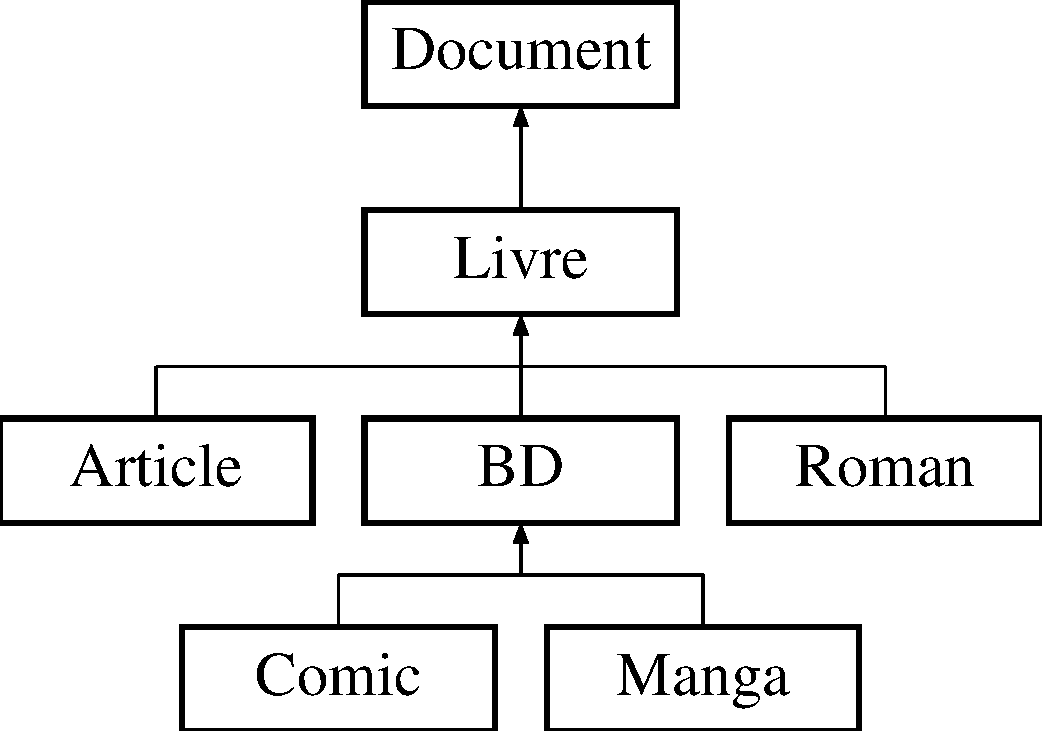
\includegraphics[height=4.000000cm]{classLivre}
\end{center}
\end{figure}
\subsection*{Public Member Functions}
\begin{DoxyCompactItemize}
\item 
\hypertarget{classLivre_adeb5fca648e4ee21494782a43a7d805f}{
void \hyperlink{classLivre_adeb5fca648e4ee21494782a43a7d805f}{setAuthor} (const std::string \&)}
\label{classLivre_adeb5fca648e4ee21494782a43a7d805f}

\begin{DoxyCompactList}\small\item\em function setAuthor who set the author of a \hyperlink{classLivre}{Livre} \item\end{DoxyCompactList}\item 
\hypertarget{classLivre_a93f7f7a6824cab47e7595018b66a882d}{
std::string \hyperlink{classLivre_a93f7f7a6824cab47e7595018b66a882d}{getAuthor} ()}
\label{classLivre_a93f7f7a6824cab47e7595018b66a882d}

\begin{DoxyCompactList}\small\item\em function getAuthor who return the author of a \hyperlink{classLivre}{Livre} \item\end{DoxyCompactList}\end{DoxyCompactItemize}
\subsection*{Protected Attributes}
\begin{DoxyCompactItemize}
\item 
\hypertarget{classLivre_a866cdec9063d1caef41471646046dfdf}{
std::string {\bfseries \_\-author}}
\label{classLivre_a866cdec9063d1caef41471646046dfdf}

\end{DoxyCompactItemize}


\subsection{Detailed Description}
class \hyperlink{classLivre}{Livre}, inheriting of class \hyperlink{classDocument}{Document} 

The documentation for this class was generated from the following files:\begin{DoxyCompactItemize}
\item 
livre.hh\item 
livre.cpp\end{DoxyCompactItemize}

\hypertarget{classManga}{
\section{Manga Class Reference}
\label{classManga}\index{Manga@{Manga}}
}


class \hyperlink{classManga}{Manga}, inheriting of class \hyperlink{classBD}{BD}  




{\ttfamily \#include $<$manga.hh$>$}

Inheritance diagram for Manga:\begin{figure}[H]
\begin{center}
\leavevmode
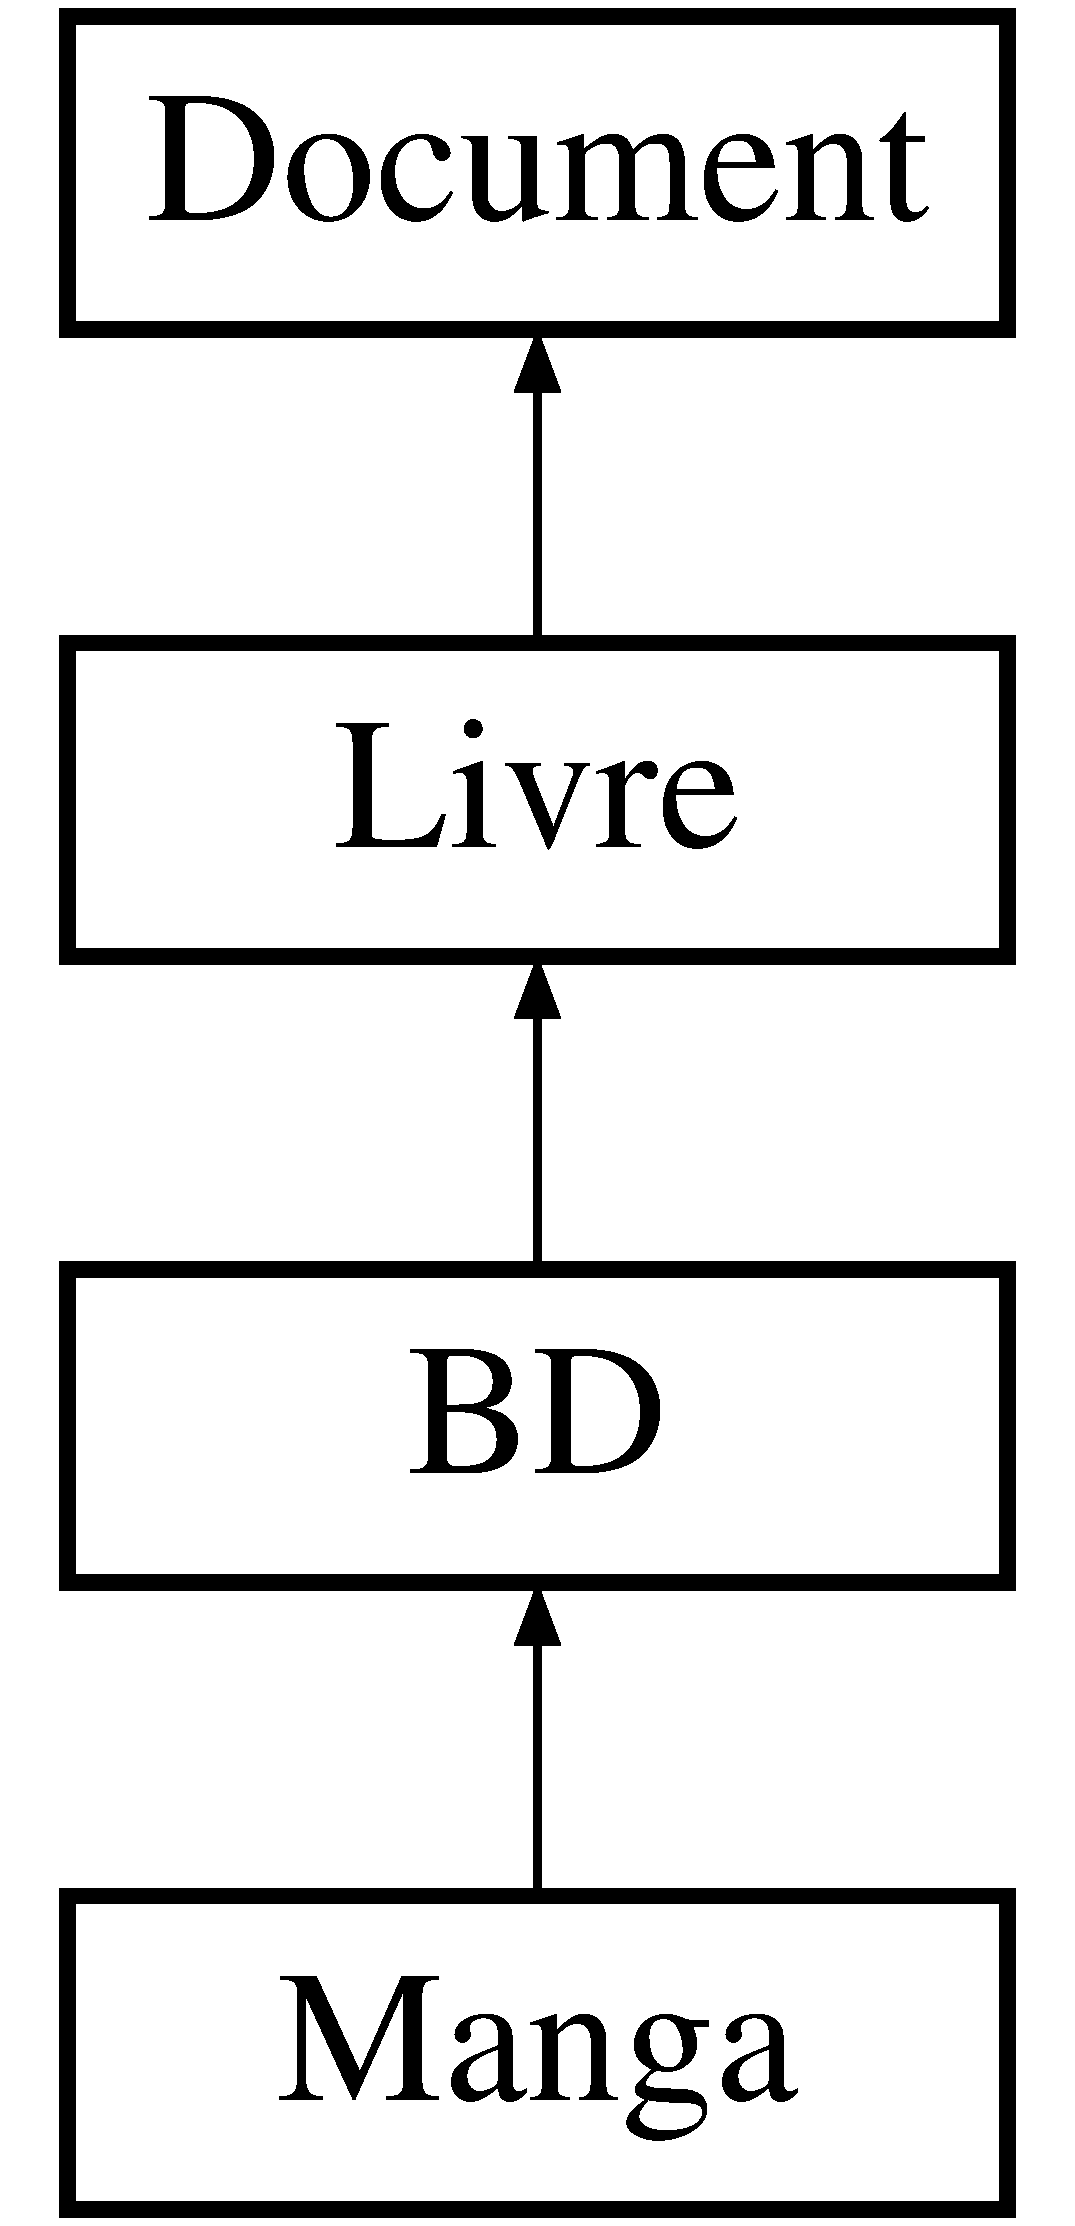
\includegraphics[height=4.000000cm]{classManga}
\end{center}
\end{figure}
\subsection*{Public Member Functions}
\begin{DoxyCompactItemize}
\item 
\hypertarget{classManga_a716ba88e31bc424d5508014887b6e019}{
void \hyperlink{classManga_a716ba88e31bc424d5508014887b6e019}{setType} (const std::string \&)}
\label{classManga_a716ba88e31bc424d5508014887b6e019}

\begin{DoxyCompactList}\small\item\em function setType who set the type of a \hyperlink{classManga}{Manga} \item\end{DoxyCompactList}\item 
\hypertarget{classManga_a3129c402dc72b73770ab9a0cc21b40f9}{
std::string \hyperlink{classManga_a3129c402dc72b73770ab9a0cc21b40f9}{getType} ()}
\label{classManga_a3129c402dc72b73770ab9a0cc21b40f9}

\begin{DoxyCompactList}\small\item\em function getType who return the type of a \hyperlink{classManga}{Manga} \item\end{DoxyCompactList}\end{DoxyCompactItemize}
\subsection*{Protected Attributes}
\begin{DoxyCompactItemize}
\item 
\hypertarget{classManga_aeefe87e43f208fcf10cb0f497f0df549}{
std::string {\bfseries \_\-type}}
\label{classManga_aeefe87e43f208fcf10cb0f497f0df549}

\end{DoxyCompactItemize}


\subsection{Detailed Description}
class \hyperlink{classManga}{Manga}, inheriting of class \hyperlink{classBD}{BD} 

The documentation for this class was generated from the following files:\begin{DoxyCompactItemize}
\item 
manga.hh\item 
manga.cpp\end{DoxyCompactItemize}

\hypertarget{classRoman}{
\section{Roman Class Reference}
\label{classRoman}\index{Roman@{Roman}}
}


class \hyperlink{classRoman}{Roman}, inheriting of class \hyperlink{classLivre}{Livre}  




{\ttfamily \#include $<$roman.hh$>$}

Inheritance diagram for Roman:\begin{figure}[H]
\begin{center}
\leavevmode
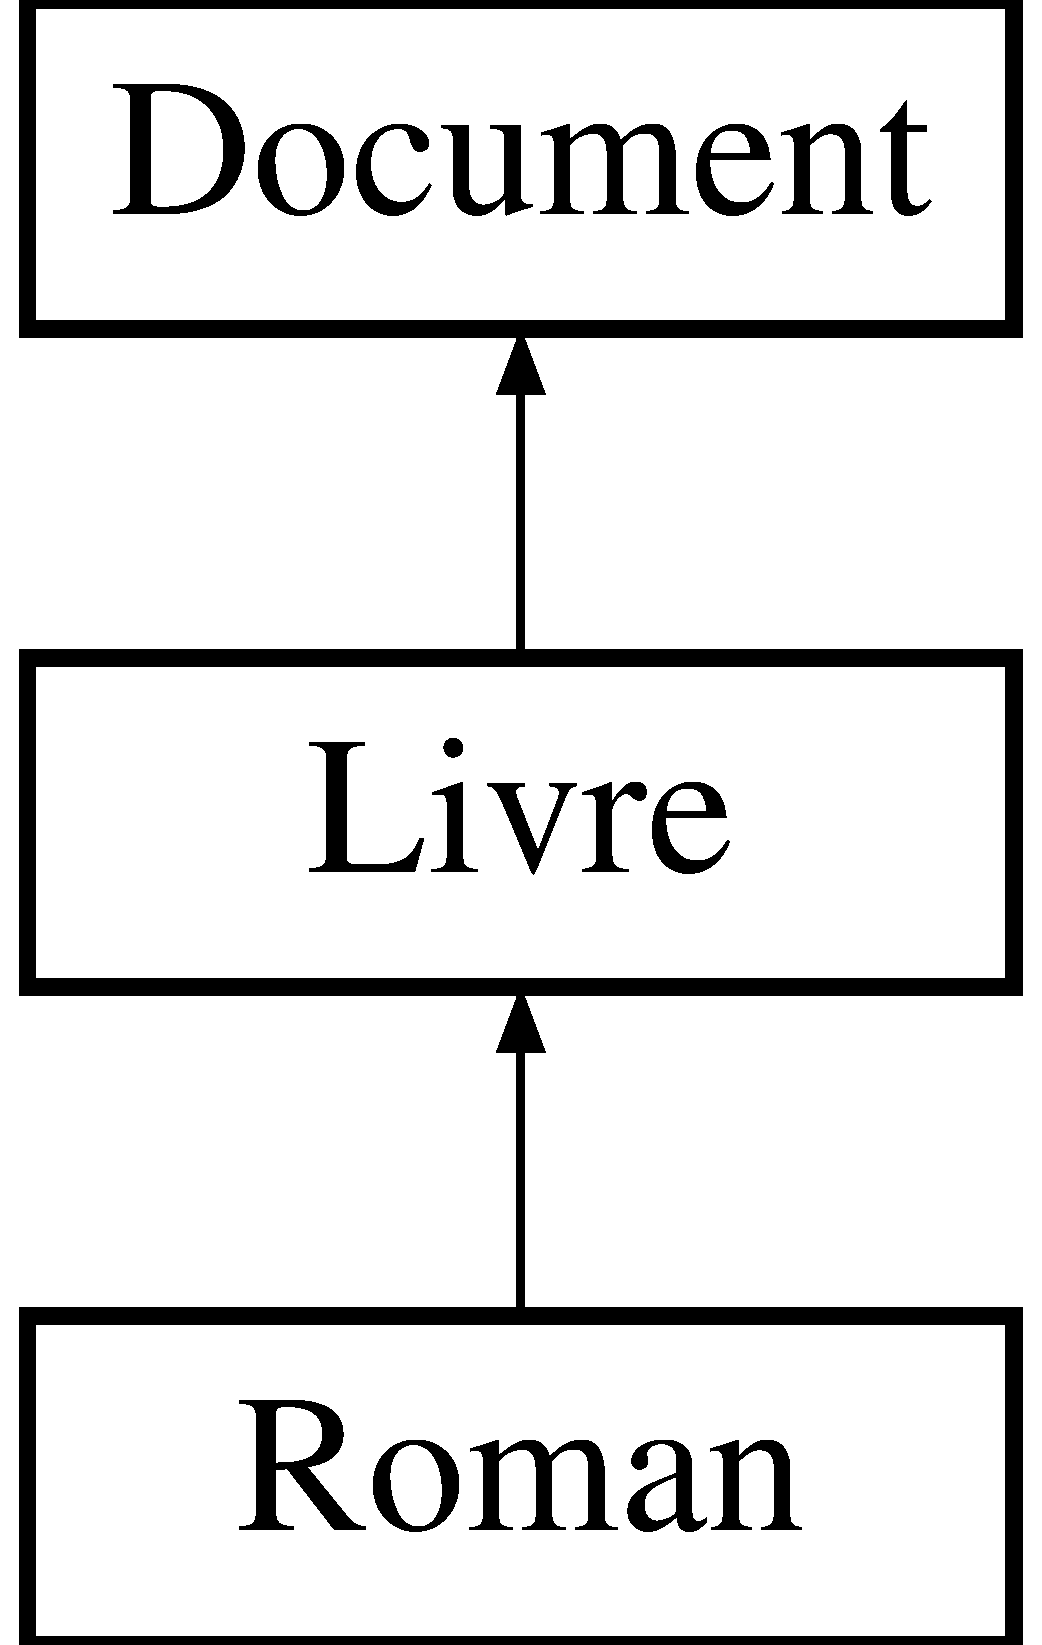
\includegraphics[height=3.000000cm]{classRoman}
\end{center}
\end{figure}
\subsection*{Public Member Functions}
\begin{DoxyCompactItemize}
\item 
\hypertarget{classRoman_a8efc9c2048221b38f90d487bd321b1dc}{
void \hyperlink{classRoman_a8efc9c2048221b38f90d487bd321b1dc}{setEditor} (const std::string \&)}
\label{classRoman_a8efc9c2048221b38f90d487bd321b1dc}

\begin{DoxyCompactList}\small\item\em function setEditor who set the Editor of a \hyperlink{classRoman}{Roman} \item\end{DoxyCompactList}\item 
\hypertarget{classRoman_a43760a779145a268fbe84222f31a08a1}{
std::string \hyperlink{classRoman_a43760a779145a268fbe84222f31a08a1}{getEditor} ()}
\label{classRoman_a43760a779145a268fbe84222f31a08a1}

\begin{DoxyCompactList}\small\item\em function getEditor who return the editor of a \hyperlink{classRoman}{Roman} \item\end{DoxyCompactList}\end{DoxyCompactItemize}
\subsection*{Protected Attributes}
\begin{DoxyCompactItemize}
\item 
\hypertarget{classRoman_a8ebd12edeb299ea1dc6b7e1706ce03dc}{
std::string {\bfseries \_\-editor}}
\label{classRoman_a8ebd12edeb299ea1dc6b7e1706ce03dc}

\end{DoxyCompactItemize}


\subsection{Detailed Description}
class \hyperlink{classRoman}{Roman}, inheriting of class \hyperlink{classLivre}{Livre} 

The documentation for this class was generated from the following files:\begin{DoxyCompactItemize}
\item 
roman.hh\item 
roman.cpp\end{DoxyCompactItemize}

\printindex
\end{document}
